\documentclass{article}
%
\usepackage{mathbbol}

\usepackage{ctex}
\usepackage{geometry}
\usepackage[dvipsnames, svgnames, x11names]{xcolor}
\usepackage[mathscr]{euscript}
\usepackage{tikz}
\usepackage{xstring}
%
\usetikzlibrary{positioning, arrows.meta, automata}
%
%
\begin{document}
%
\begin{center}
  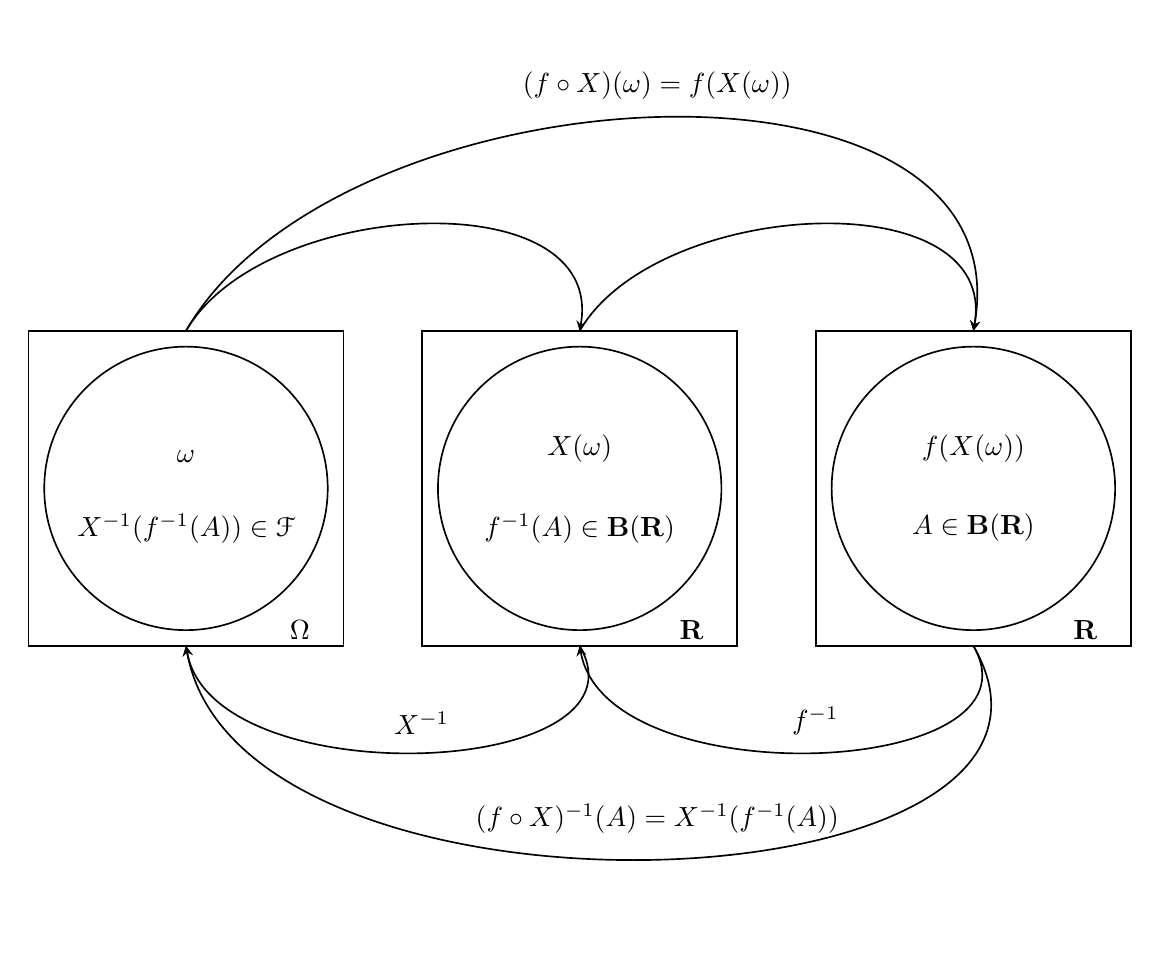
\begin{tikzpicture}[->,>=stealth,node distance=2cm,semithick,initial text=,]
    
  \draw[-] (-2,-2) rectangle (2,2);
  \draw[-] (0,0) circle (1.8);
  \draw[-] (0,0) node [above = 0.2cm]{${X(\omega)}$};
  \draw[-] (0,0) node [below = 0.2cm]{${f^{-1}(A)\in\mathbf{B}(\mathbf{R})}$};
  \draw[-] (1.8,-1.8) node [left = 0.1cm]{${\mathbf{R}}$};

  \tikzset{shift={(-5,0)}};
  \draw[-] (-2,-2) rectangle (2,2);
  \draw[-] (0,0) circle (1.8);
  \draw[-] (0,0) node [above = 0.2cm]{${\omega}$};
  \draw[-] (0,0) node [below = 0.2cm]{${X^{-1}(f^{-1}(A))\in\mathscr{F}}$};
  \draw[-] (1.8,-1.8) node [left = 0.1cm]{${\Omega}$};


  \tikzset{shift={(10,0)}};
  \draw[-] (-2,-2) rectangle (2,2);
  \draw[-] (0,0) circle (1.8);
  \draw[-] (0,0) node [above = 0.2cm]{${f(X(\omega))}$};
  \draw[-] (0,0) node [below = 0.2cm]{${A\in\mathbf{B}(\mathbf{R})}$};
  \draw[-] (1.8,-1.8) node [left = 0.1cm]{${\mathbf{R}}$};

  \draw[->] (0, -2) to[out=-60, in=-80] node[above=0.1cm]{${f^{-1}}$} (-5,-2);
  \draw[->] (-5, -2) to[out=-60, in=-80] node[above=0.1cm]{${X^{-1}}$} (-10,-2);
  \draw[->] (0, -2) to[out=-60, in=-80] node[above=0.2cm]{${(f\circ X)^{-1}(A)=X^{-1}(f^{-1}(A))}$} (-10,-2);
  \draw[->] (-5, 2) to[out=60, in=80] node[above=0.1cm]{} (0,2);
  \draw[->] (-10, 2) to[out=60, in=80] node[above=0.1cm]{} (-5,2);
  \draw[->] (-10, 2) to[out=60, in=80] node[above=0.1cm]{$(f\circ X)(\omega)=f(X(\omega))$} (0,2);
  

  \end{tikzpicture}
  \heiti\\ 图8.10 复合随机变量\songti
\end{center}
%
\end{document}
